% Copyright Ben Paul Wise. All Rights Reserved.
% The standard sheet at 75 km: shared by circling_dragons_map_and_rules_V3.tex and maneuver_studies_75km.tex,
% each of which gives the heading.  Needs the labels sec:maneuvers and sub:mrules (maneuver-studies.tex).
The standard sheet has 75 km between hex centers. It replaced the first sheet, at 100 km, in October 2026, because at 100 km the Hunan corridor is too narrow for two maneuvers that decided its battles: Xue Yue's defense of Changsha in 1939--42 and the Japanese envelopment of Hengyang in 1944 (section~\ref{sec:maneuvers}).

Both sheets cover the same area and are built by the same programs from the same sources, so the scale is a setting of the build and the first sheet can still be produced for comparison. Every ruling made on the 100 km sheet was carried over: the named mountain ranges, the lakes and the Tonghua redoubt are lists of 100 km hexes, and each 75 km hex whose center falls in a listed hex takes the ruling. Three coastal hexes, each just under half land, were ruled land so that the railways of the Liaodong peninsula, the south shore of Hangzhou Bay and the Korean west coast stay on land. At Yueyang the Yangtze was moved to the north side of the city's hex, so that the railway south to Changsha does not cross it. Between Tongguan and Zhengzhou the Yellow River was moved to the north side of the Sanmenxia and Luoyang hexes, so that the Longhai railway stays on the south bank and crosses the river only on its 1938--47 course east of Zhengzhou. The Ussuri was extended two hexsides to join the Amur at Khabarovsk. The sheet passes the same validation and network checks as the first one.

\begin{center}
\begin{tabular}{lrr}
\toprule & First sheet & Standard sheet \\\midrule
Distance between hex centers & 100 km & 75 km \\
Columns by rows & 35 by 34 & 47 by 46 \\
Hexes on the sheet & 1,190 & 2,162 \\
Hexes in play (China, Manchukuo, Korea) & 672 & 1,187 \\
Mongolian hexes, open to Soviet formations only & 131 & 242 \\
Clear hexes across the corridor at Changsha & 2 & 3 \\
Clear hexes across the corridor at Hengyang & 2 & 3 \\
Hexes from Yueyang to Changsha & 1 & 2 \\
Hexes from Hankow to Dushan along the corridor & 12 & 15 \\
Sheet size with 3/4 inch hexes & 24 by 27 in & 32 by 36 in \\
\bottomrule
\end{tabular}
\end{center}

Of the hexes in play, the two sheets have nearly the same terrain: clear 26 and 27 percent, broken 33 and 32, mountain 24 and 23, steppe 15 and 15, marsh 3 and 3. The smaller hex does not make the country look flatter, so the terrain thresholds were left unchanged.

The standard sheet adds one line class, the \textbf{minor river}, drawn thinner than the major rivers and printed only where a minor river shaped a campaign. Two are printed: the Xinqiang and the Miluo, the delay lines north of Changsha on which Xue Yue's screens stood. Each crosses the railway column and the lane east of it, and each runs into the Xiang. The Laodao, the third of his lines, lies inside the Changsha hex and is not printed. In the provisional rules a minor river costs less to cross than a major river, and a formation behind one may withdraw before combat (section~\ref{sub:mrules}).

At 3/4 inch hexes the sheet is about 32 by 36 inches and fits on two 22 by 34 inch map sheets joined along their long edges. To keep the density of pieces of the first estimate, the counter set was grown to 126 unit pieces and 250 counters in all.

\begin{figure}[p]\centering
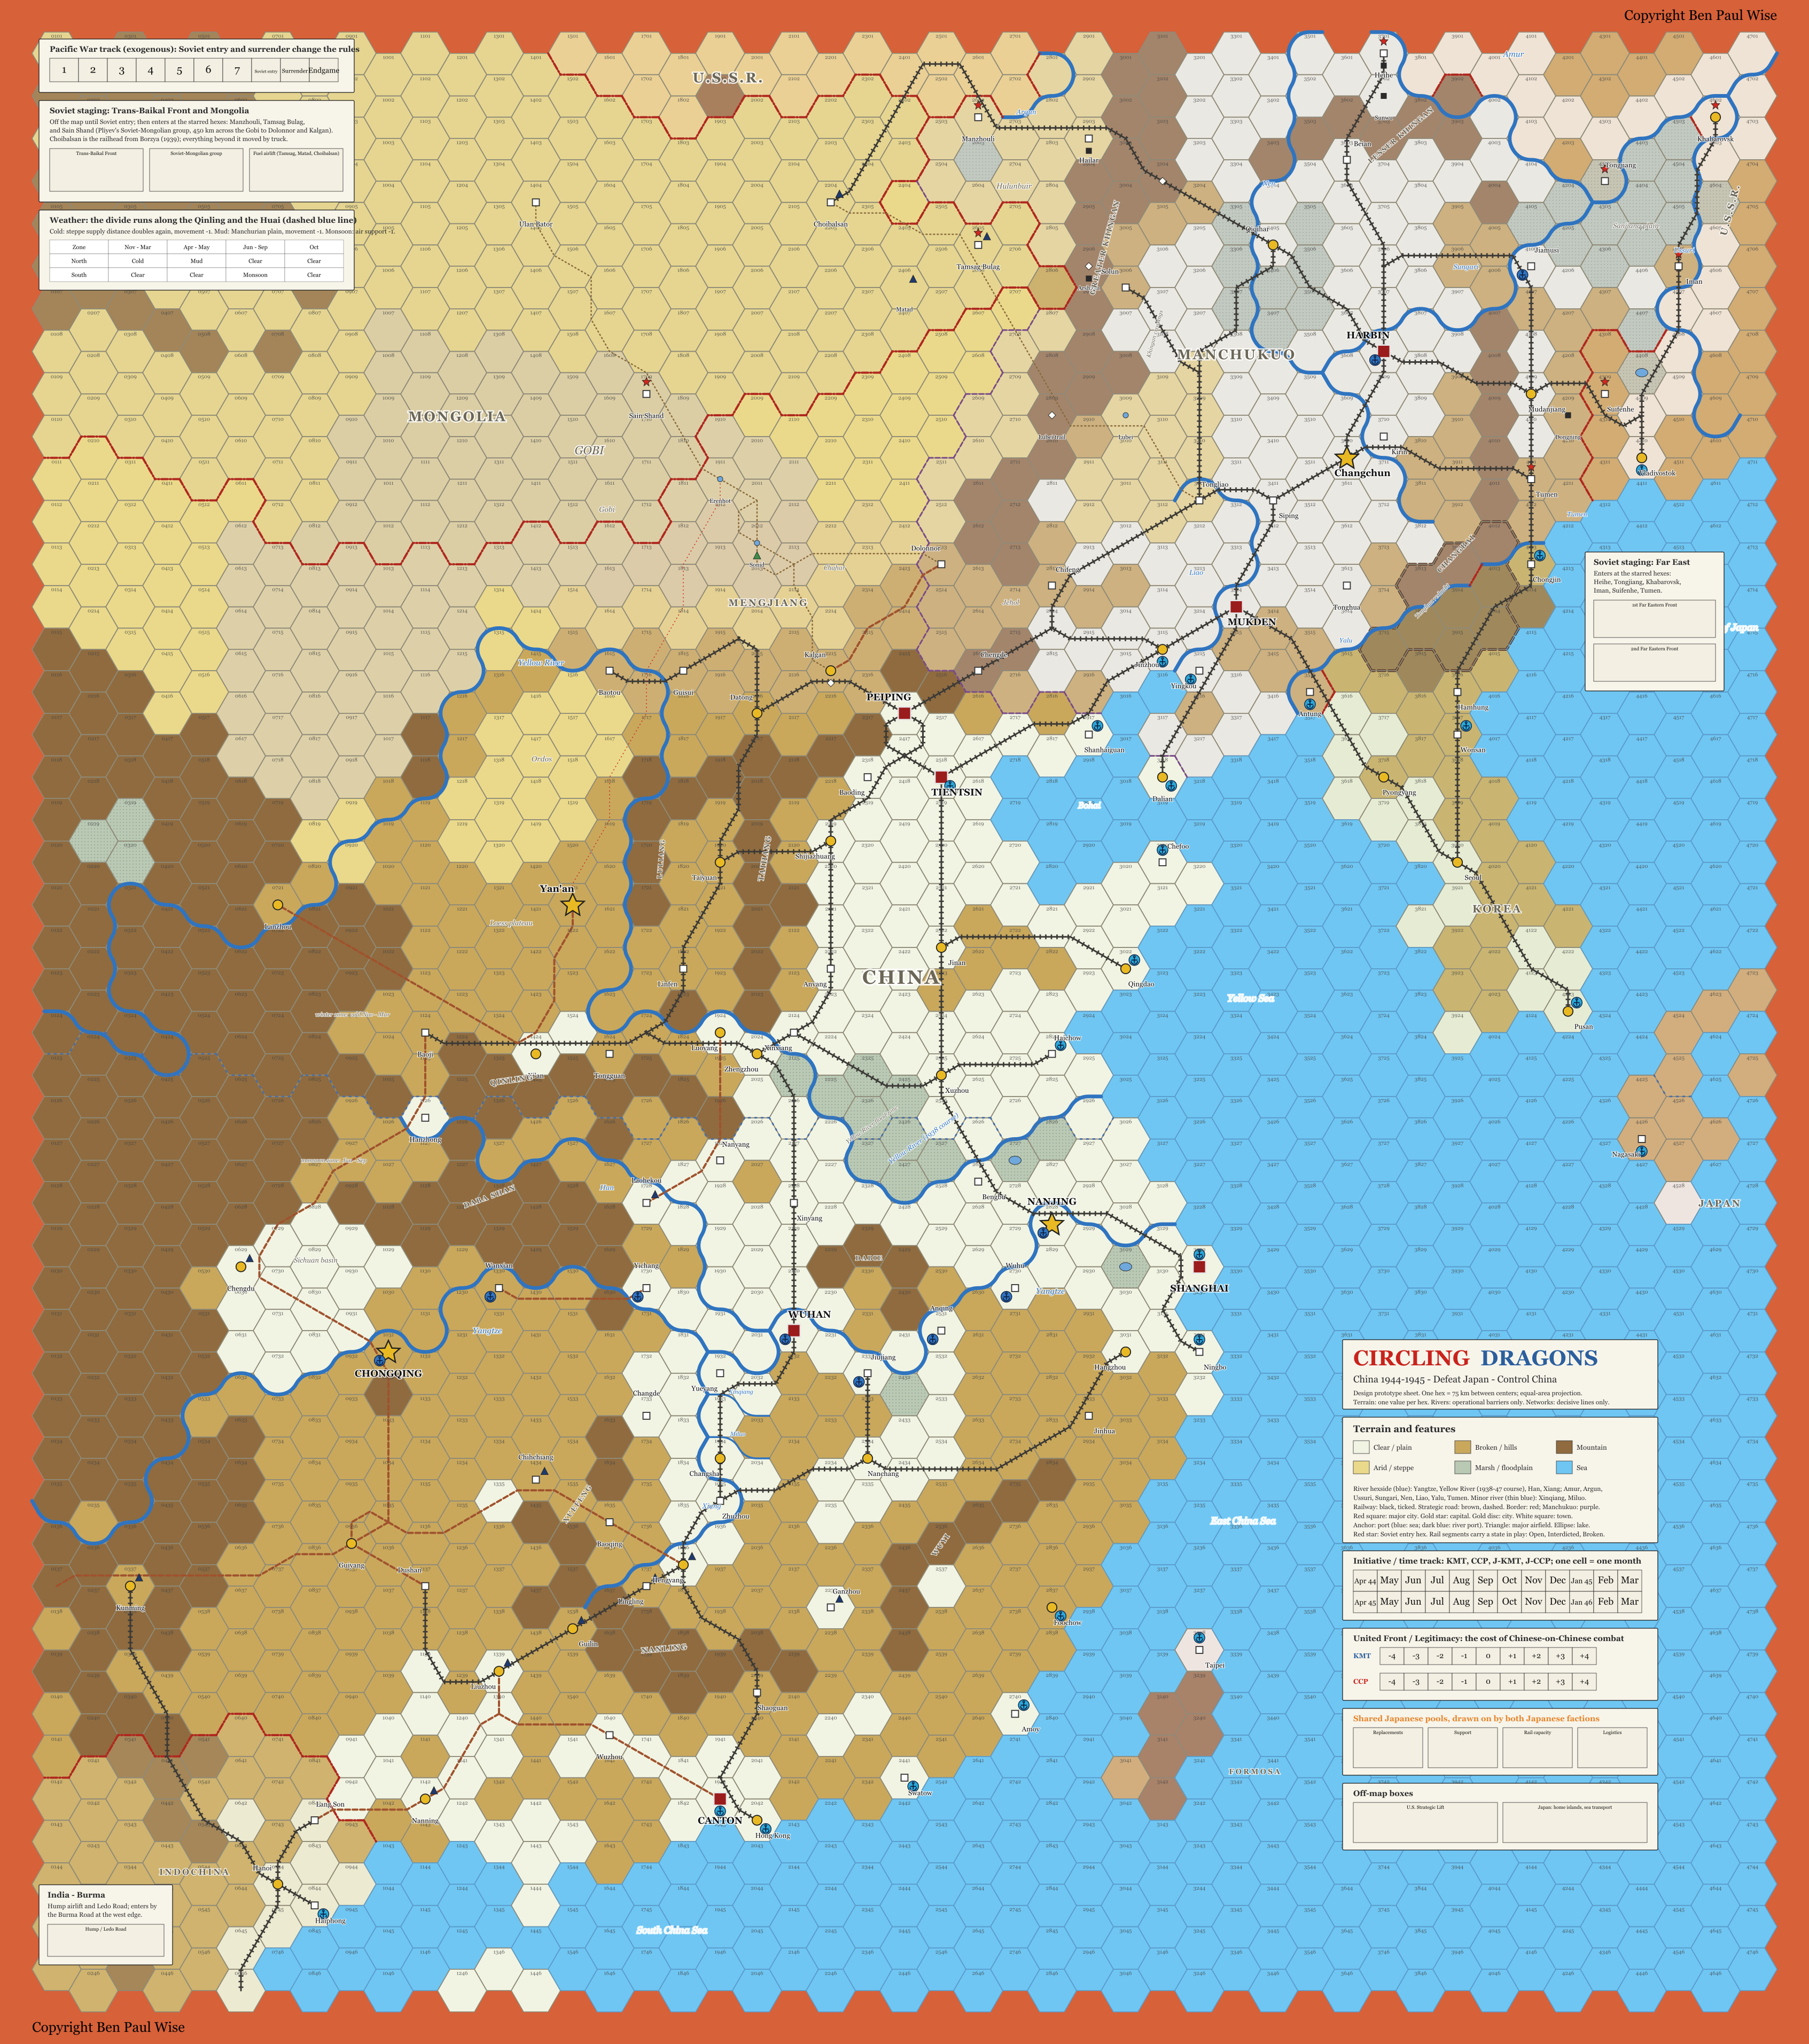
\includegraphics[width=\textwidth,height=.86\textheight,keepaspectratio]{../map_graphics/xml/circling-dragons.png}
\caption{The standard sheet, 75 km between hex centers. The furniture panels keep their size and their places in the corners where little fighting took place; the Mongolian features and the political layer are those of the first sheet.}
\end{figure}
% Copyright Ben Paul Wise. All Rights Reserved.
